\subsection{Praxistest: Zwei Tage im Filmstudio}

Am Montagmorgen stand ich vor dem Albrecht-Ade-Studio der Filmakademie Ludwigsburg. Die große Soundstage ist professionell ausgestattet. In wenigen Stunden würde hier im Produktionssetting getestet werden, ob M.A.S.K. dem Druck einer echten Filmproduktion standhalten konnte.

\begin{figure}[h]
   \centering
   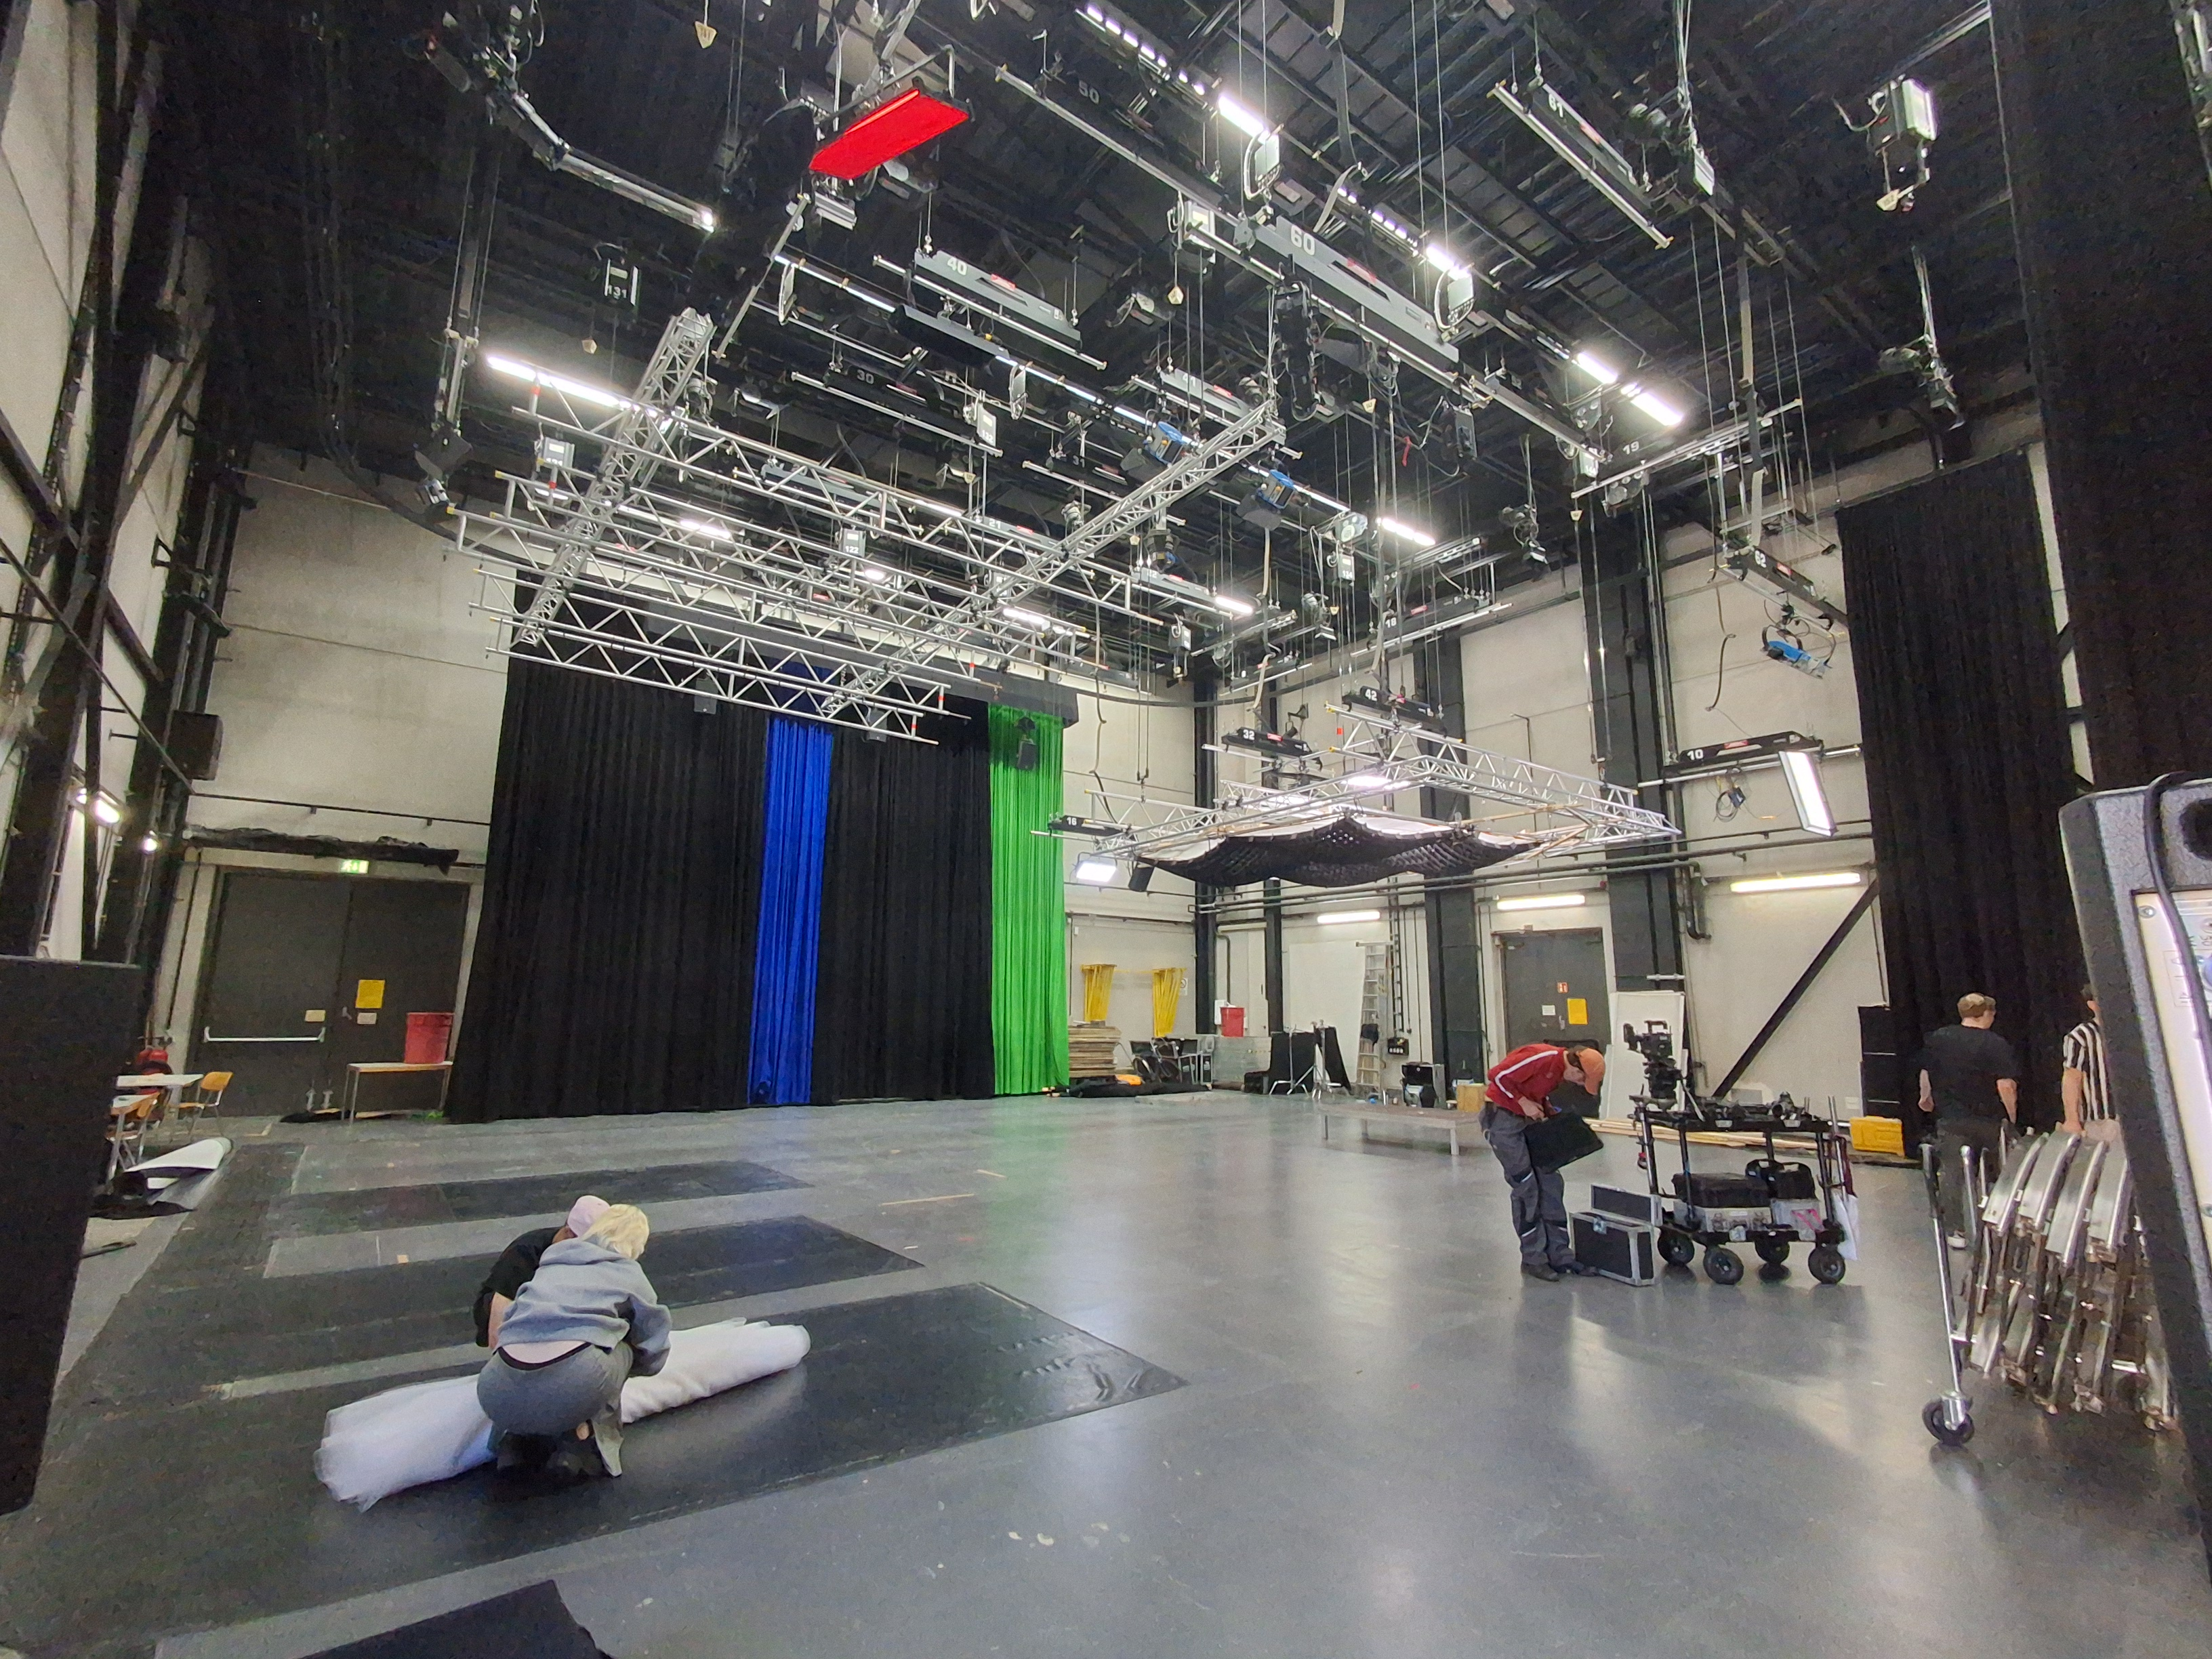
\includegraphics[width=0.9\textwidth]{images/onSetImages/InsideWideshotAlbrechtAdeStudio.jpg}
   \caption{Albrecht-Ade-Studio: Erste Eindrücke der großen Soundstage vor Produktionsbeginn}
   \label{fig:studio_interior}
\end{figure}

Das technische Setup verlief gut – die Proben hatten sich ausgezahlt. Schnell waren Kinect, Beamer und TouchDesigner einsatzbereit. Die eigentliche Herausforderung begann mit den Abstimmungen zwischen Kamerateam, Lichtcrew, Producern und Directors. Jede Kameraposition bedeutete neue Offset-Kalibrierungen, da der Tänzer bewusst Abstand zu den projizierten Visuals hielt. Was in der Theorie einfach klang – Parameter anpassen, fertig – wurde zur geduldigen Arbeit zwischen den Takes.

\begin{figure}[h]
   \centering
   \includegraphics[width=0.9\textwidth]{images/onSetImages/MartyBehindTheStudioCurtainDoingTouchDesigner.jpg}
   \caption{Technische Umsetzung: TouchDesigner-Bedienung hinter dem Studievorhang während der Produktion}
   \label{fig:technical_operation}
\end{figure}

\newpage

\subsection{Tag 1: Die drei Systeme im Einsatz}

\subsubsection{Spike-System: Funktionstest}

Das 64-Spike-System machte den Anfang. Die Overhead-Kamera blickte von der Decke auf den Tänzer, während 64 radiale Segmente auf dem Boden projiziert wurden. Die wenige Tage alte Infrarot-Lösung bewährte sich: Trotz intensiver Beamer-Beleuchtung erkannte MediaPipe den Tänzer mit einer Genauigkeit, bei der man keine Fehler merkte.

\begin{figure}[h]
   \centering
   \includegraphics[width=0.9\textwidth]{images/onSetImages/wideStudioShotPreparingTopDownSpikeShot.jpg}
   \caption{Studio-Vorbereitung: Setup für Top-Down-Spike-System mit Overhead-Kamera-Positionierung}
   \label{fig:topdown_setup}
\end{figure}

Die Geschichte hinter der Infrarot-Lösung war kurz: Maja und Rahel hatten mir während eines Wanderausflugs eine WhatsApp geschickt – das RGB-Tracking versagte unter Beamer-Licht. Beim Laufen kam die Eingebung: OBS Virtual Camera könnte den Kinect-Infrarot-Stream als Kameraeingang ausgeben. Nach der Wanderung folgte die Umsetzung: Plugin suchen, DLL installieren, Technical Rider schreiben. Die Lösung war unkonventionell, aber sie funktionierte.

\begin{figure}[h]
   \centering
   \includegraphics[width=0.9\textwidth]{images/onSetImages/cameraBTSPicofACameraScreenOfTopDown64SpikeOfDancerOnFloor.jpg}
   \caption{Kameramonitor: Top-Down-Aufnahme des 64-Spike-Systems mit Tänzer auf dem Studioboden}
   \label{fig:camera_monitor}
\end{figure}

\begin{figure}[h]
   \centering
   \includegraphics[width=0.9\textwidth]{images/production/spike_system_in_action.jpg}
   \caption{Spike-System in Aktion: Reagiert präzise auf Hand- und Fußbewegungen}
   \label{fig:spike_action}
\end{figure}

Das Spike-System lief ohne einen einzigen Aussetzer. Die hohe Winkelauflösung reichte aus, um selbst subtile Handbewegungen in präzise Spike-Aktivierungen zu übersetzen. Nach wenigen Takes war die Sequenz im Kasten.

\newpage

\subsubsection{Kopfpartikel: Die Geduldsprobe}

Das Kopfpartikel-System war die schwierigste Aufgabe. Frontale Kamera, RGB-Modus (Infrarot funktionierte aus diesem Winkel nicht), Beamer von hinten – eine Konstellation, die MediaPipe an seine Grenzen brachte.

\begin{figure}[h]
   \centering
   \includegraphics[width=0.9\textwidth]{images/production/head_particles_setup_diagram.jpg}
   \caption{Kopfpartikel-Setup: Komplexe Kamera-Beamer-Ausrichtung}
   \label{fig:head_setup}
\end{figure}

Die Beleuchtung erwies sich als unzureichend für die RGB-basierte Skelett-Erkennung von MediaPipe. Nach mehreren fehlgeschlagenen Tracking-Versuchen wurde das Lichtteam gebeten, die Ausleuchtung zu verstärken. Diese Anpassung war essentiell für die Funktionsfähigkeit des Systems, da MediaPipe auf ausreichende Beleuchtung für die Bildanalyse angewiesen ist. Das Lichtteam setzte die Anforderung professionell um.

\begin{figure}[h]
   \centering
   \includegraphics[width=0.9\textwidth]{images/onSetImages/PictureOfDancerBTSinSetupForHeadTrackingBubbles.jpg}
   \caption{Kopfpartikel-Setup: Tänzer bei Vorbereitung für Head-Tracking mit kritischen Lichtbedingungen}
   \label{fig:dancer_head_tracking}
\end{figure}

\begin{figure}[h]
   \centering
   \includegraphics[width=0.9\textwidth]{images/production/head_particles_low_light.jpg}
   \caption{Schwierige Bedingungen: MediaPipe kämpft mit schlechtem Licht}
   \label{fig:low_light_tracking}
\end{figure}

Ein weiteres Problem: Der Kameramann stand im Sichtfeld der Kinect. In den meisten Momenten war das in Ordnung, da ich MediaPipe auf ein einzigen Körper parametisiert hatte, aber falls der Tänzer nicht vor dem Kamermann begonnen wurde zu tracken, oder es zu einem kurzen Aussetzer kommt, kam es manchmal dazu, dass der Kameramann getrackt wurde.

Nach mehreren Takes und unzähligen Mikro-Anpassungen hatten wir die Sequenz. Die Partikel folgten dem Kopf, wechselten die Zustände wenn die Hände über die Schultern gingen, und die Projektion passte endlich zur Kameraposition.

\begin{figure}[h]
   \centering
   \includegraphics[width=0.9\textwidth]{images/production/head_particles_result.jpg}
   \caption{Endergebnis: Trotz Herausforderungen ein gutes Resultat}
   \label{fig:head_result}
\end{figure}

\subsubsection{Hand-Feuer: Wenn Effekte zu gut funktionieren}

Nach der Mittagspause – es gab selbstgemachtes Curry, was die anfangs ungeduldige Kameracrew merklich aufheiterte – folgte nach einem kurzen finish der Head-Partikel das Hand-Feuer-Setup. Die modulare Architektur erwies sich als vorteilhaft: Das System war in wenigen Minuten einsatzbereit.

\begin{figure}[h]
   \centering
   \includegraphics[width=0.9\textwidth]{images/production/hand_fire_setup.jpg}
   \caption{Hand-Feuer Setup: Modulare Architektur bewährt sich}
   \label{fig:hand_fire_setup}
\end{figure}

Der erste Take verlief problematisch. Die blauen Flammen folgten den Händen so präzise, dass der Kameramann mit seinem Zugwagen den Effekten folgte – und dabei den Tänzer aus dem Frame verlor. Die Visuals funktionierten zu gut für die geplante Kameraführung.

Dann kam die Stoff-Sequenz. Niemand hatte erwähnt, dass der Tänzer sich in durchsichtigen weißem Stoff hüllen würde. Der Stoff verschleierte die Körperform so effektiv, dass MediaPipe sofort das Skelett-Tracking verlor. Panik? Nicht wirklich. Die Debug-Visualisierung auf dem zweiten Monitor zeigte genau, wann MediaPipe den Tänzer wieder erkannte. Im richtigen Moment aktivierten wir die Effekte per Tastatur-Shortcut. Nicht elegant, aber funktional, und ein Einsetzen der Hand-Magie konnte in dem Moment getriggert werden, wenn der Tänzer sich aus dem Stoff befreit hat und die Arme ausstreckt.

\begin{figure}[h]
   \centering
   \includegraphics[width=0.9\textwidth]{images/production/hand_fire_in_action.jpg}
   \caption{Hand-Feuer in Aktion: Blaue Partikel folgen den Händen}
   \label{fig:hand_fire_action}
\end{figure}

\subsection{Tag 2: Dokumentation und Reflexion}

Der zweite Tag fokussierte sich auf traditionelle Filmaufnahmen ohne interaktive Systeme. Neben der Dokumentation durch Behind-the-Scenes-Fotografie unterstützte ich das Team bei verschiedenen Produktionsaufgaben, einschließlich der Bedienung der studioeigenen Zugmaschine. Die Production Assistants vermittelten wertvolle Einblicke in die professionelle Studiotechnik. Trotz gelegentlicher organisatorischer Unterbrechungen zwischen den Aufnahmen verlief der Tag produktiv.

\begin{figure}[h]
   \centering
   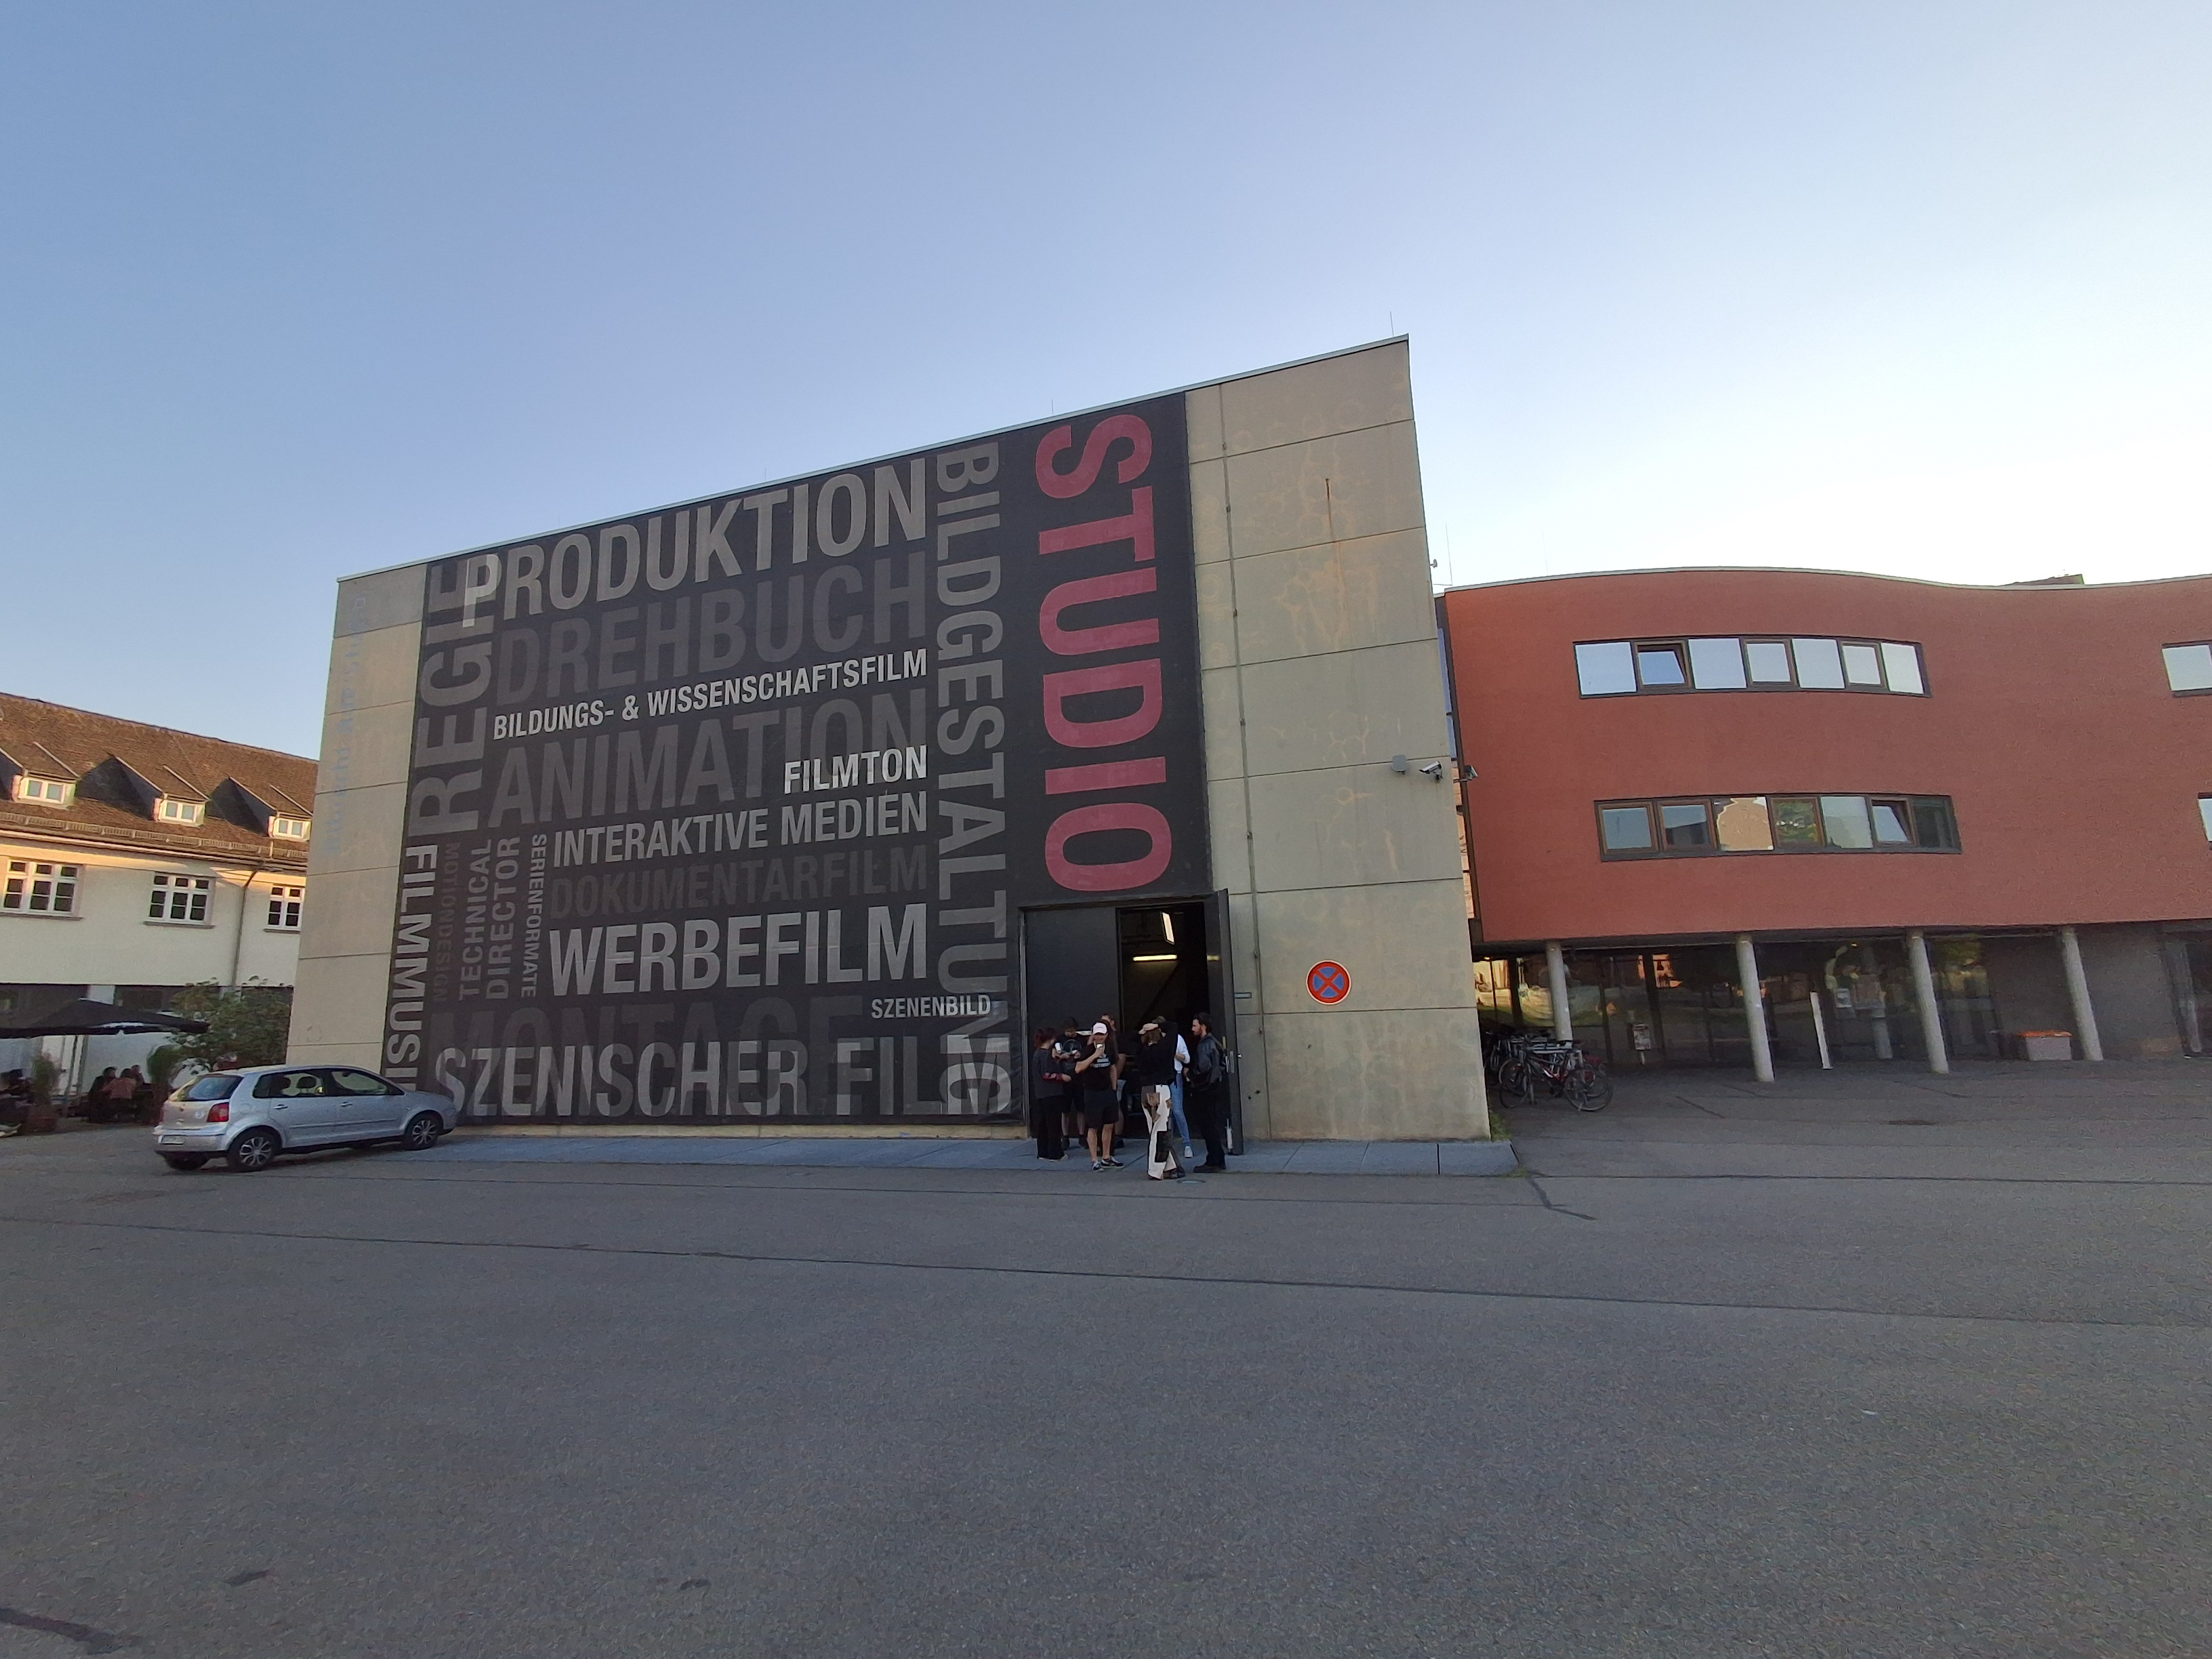
\includegraphics[width=0.9\textwidth]{images/onSetImages/WideShotOfOutsideOfStudioAfter2DayShoot.jpg}
   \caption{Produktionsabschluss: Außenansicht des Albrecht-Ade-Studios nach zweitägiger Drehzeit}
   \label{fig:studio_exterior}
\end{figure}

\begin{figure}[h]
   \centering
   \includegraphics[width=0.9\textwidth]{images/production/crew_setup_wide.jpg}
   \caption{Teamarbeit: Professionelle Crew integriert M.A.S.K. in den Workflow}
   \label{fig:crew_setup}
\end{figure}

Maja und Rahel, die Directors, waren durchgehend gestresst aber sehr freundlich. Ihre Energie war ansteckend – sie glaubten an das Projekt, auch wenn die Technik manchmal zickte. Das Team war größer als erwartet, professioneller als befürchtet, und am Ende des Tages folgten wir uns alle auf Instagram.

\begin{figure}[h]
   \centering
   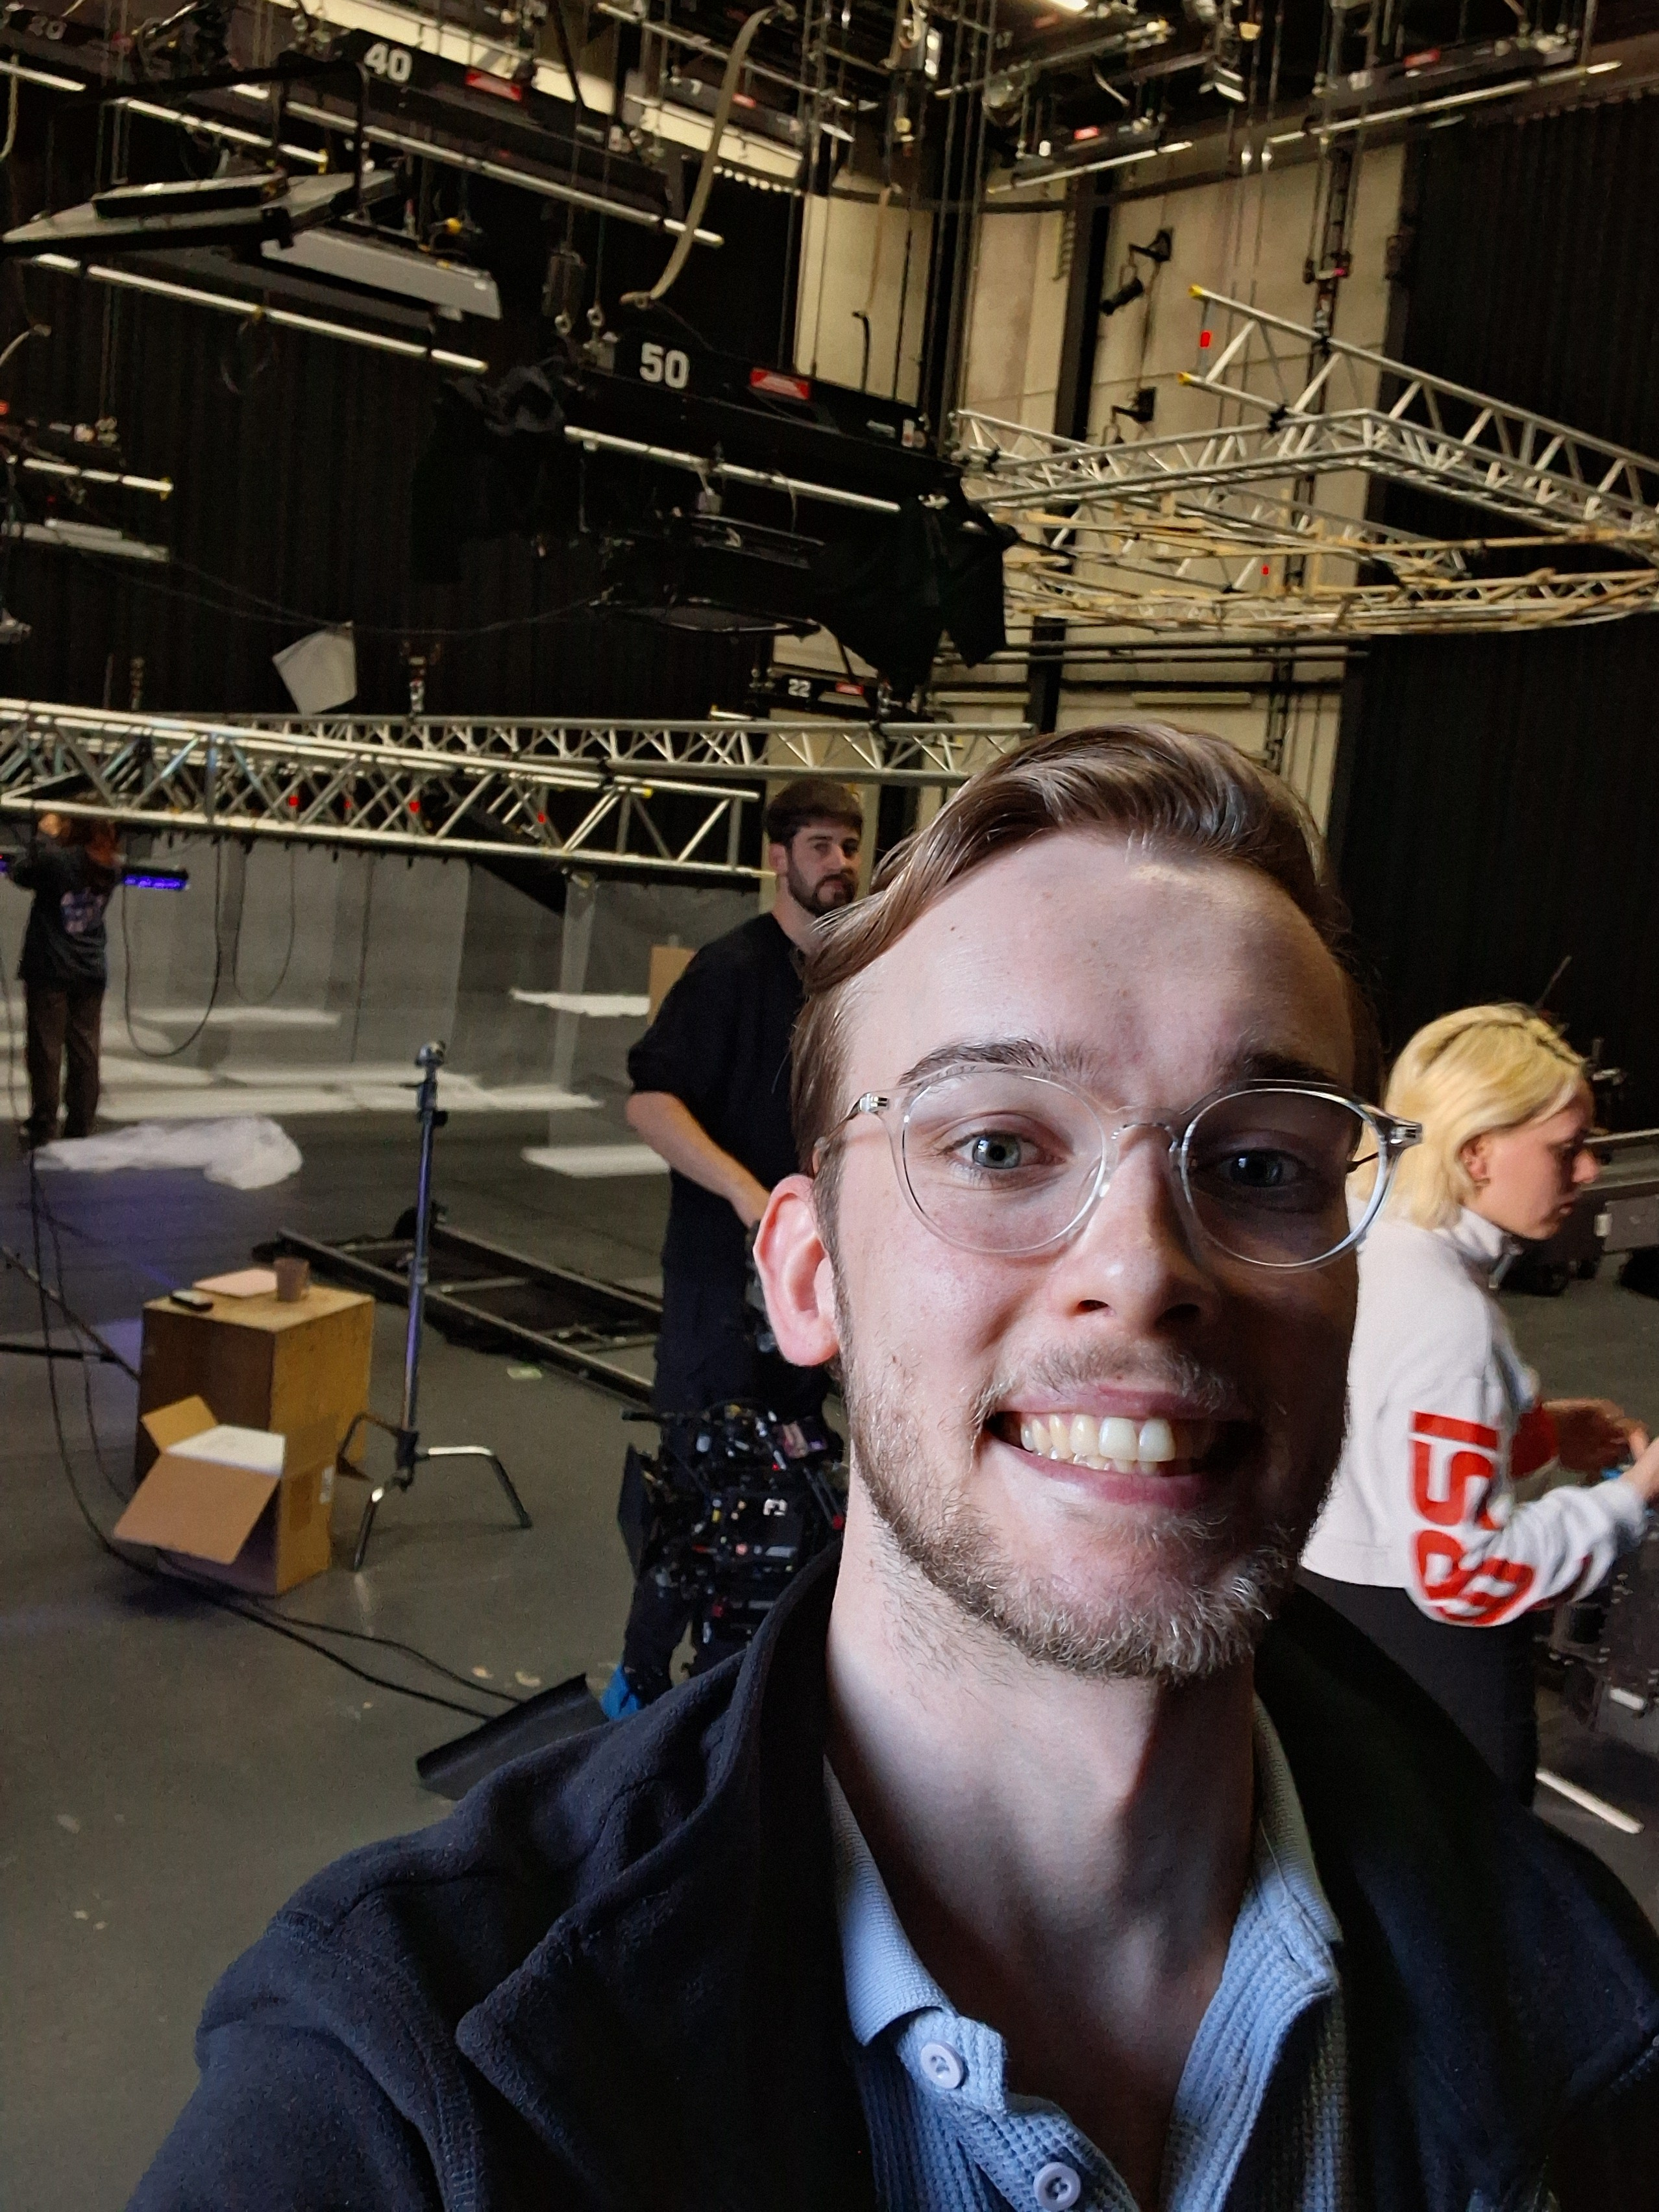
\includegraphics[width=0.9\textwidth]{images/onSetImages/MartySmileyIntoCameraOnSet.jpg}
   \caption{Teamdynamik: Entspannte Atmosphäre zwischen den Takes trotz technischer Herausforderungen}
   \label{fig:team_atmosphere}
\end{figure}

\begin{figure}[h]
   \centering
   \includegraphics[width=0.9\textwidth]{images/production/studio_wide_angle.jpg}
   \caption{Albrecht-Ade-Studio: Professionelle Soundstage}
   \label{fig:studio_wide}
\end{figure}

\newpage

\subsection{Ehrliche Bilanz}

Nach zwei Tagen Produktion mit umfangreichem 4K-Material stand fest: M.A.S.K. hatte seinen ersten echten Praxistest bestanden. Die Infrarot-Lösung erwies sich als wirksam, das 64-Spike-System lief zuverlässig, und selbst die problematischen RGB-Modi lieferten am Ende brauchbare Ergebnisse.

\textbf{Was gut lief:}
\begin{itemize}
   \item Die Infrarot-Lösung eliminierte die Beleuchtungsprobleme vollständig
   \item Das 64-Spike-System arbeitete über Stunden hinweg sehr zuverlässig
   \item Alle Setups waren schnell einsatzbereit
   \item Kein einziger System-Absturz während der gesamten Produktion
   \item Die modulare Architektur ermöglichte schnelle Anpassungen
\end{itemize}

\textbf{Was schwierig war:}
\begin{itemize}
   \item Head-Particle-Modi erforderten konstante Rekalibrierung bei Positionswechseln
   \item Schwaches Licht degradierte die Tracking-Performance erheblich
   \item Live-Debugging unter Zeitdruck testete die Nerven
   \item Extreme Verdeckungen (durchsichtiger Stoff) überforderten MediaPipe
   \item Die eigene Stimme zu finden und technische Bedürfnisse zu kommunizieren
\end{itemize}

\textbf{Finale Metriken:}
\begin{itemize}
   \item \textbf{Setup-Zeit:} Kurze Zeit pro System (inklusive Kalibrierung)
   \item \textbf{Tracking-Zuverlässigkeit:} Sehr hoch (Infrarot), gut (RGB bei ausreichend Licht)
   \item \textbf{Takes pro Sequenz:} Wenige (Spike-System), mehrere (Kopfpartikel), einige (Hand-Feuer)
   \item \textbf{Datenvolumen:} Umfangreiches 4K-Material
   \item \textbf{Crew-Integration:} Nach anfänglicher Skepsis volle Akzeptanz
   \item \textbf{Gesamtkosten:} Kostengünstige Hardware + kostenlose Software
\end{itemize}